\documentclass[
	letterpaper, % Paper size, specify a4paper (A4) or letterpaper (US letter)
	10pt, % Default font size, specify 10pt, 11pt or 12pt
]{CSUniSchoolLabReport}

%----------------------------------------------------------------------------------------
%	REPORT INFORMATION
%----------------------------------------------------------------------------------------

\title{Lab Two\\ Fundamentals of Electronics \\ EECE2412/3} % Report title

\author{Michael \textsc{Brodskiy}\\ \small \href{mailto:Brodskiy.M@Northeastern.edu}{Brodskiy.M@Northeastern.edu}}

\date{October 15, 2024} % Date of the report

%----------------------------------------------------------------------------------------


\begin{document}

\maketitle % Insert the title, author and date using the information specified above

\begin{center}
	\begin{tabular}{l r}
		Date Performed: & October 1/8, 2024 \\ % Date the experiment was performed
        Partner: & Rahul \textsc{Singh} \\ % Partner names
		Instructor: & Professor \textsc{Onabajo} \\ % Instructor/supervisor
        TAs: & Ming \textsc{Xiang} \& Amr \textsc{Kassab} \\ % Teachers Assistants 
	\end{tabular}
\end{center}

\newpage

\begin{abstract}

  The goal of this laboratory experiment is to introduce the performer to several different types of pn-junction diodes, which include silicon/germanium junction diodes, light-emitting diodes (LEDs), and zener diodes. A custom circuit is then designed to turn on/off various LEDs at specified voltages.

\end{abstract}

\begin{flushleft}

  \textsc{Keywords:} \underline{pn-junction}, \underline{diode}, \underline{silicon/germanium}, \underline{LED}, \underline{zener}

\end{flushleft}

\newpage

\tableofcontents
\listoffigures

\newpage

\section{Equipment}

Available equipment included:\\

\begin{itemize}

  \item Basic Circuit Components (Capacitors, Resistors, Inductors, etc.)

  \item Keysight EDU36311A Dual DC Power Supply

  \item Keysight EDU33212A Function Generator

  \item Keysight DSOX1204G Digital Oscilloscope

  \item BNC Cables

  \item A Variety of Diodes (1N914 Si Diode, 1N34A Ge Diode, 1N4735A Zener Diode, etc.)

\end{itemize}

\newpage

\section{Performing the Experiment}

\subsection{Basic Diode Test}

We begin with the construction of a simple circuit to test a 1N914 Si Diode:

\begin{figure}[H]
  \centering
  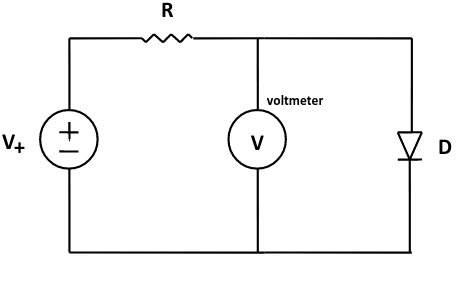
\includegraphics[width=.75\textwidth]{Figures/L2F1}
  \caption{Circuit Schematic for Part 1}
  \label{fig:1}
\end{figure}

The physical construction is shown in Figure \ref{fig:2} below:

\begin{figure}[H]
  \centering
  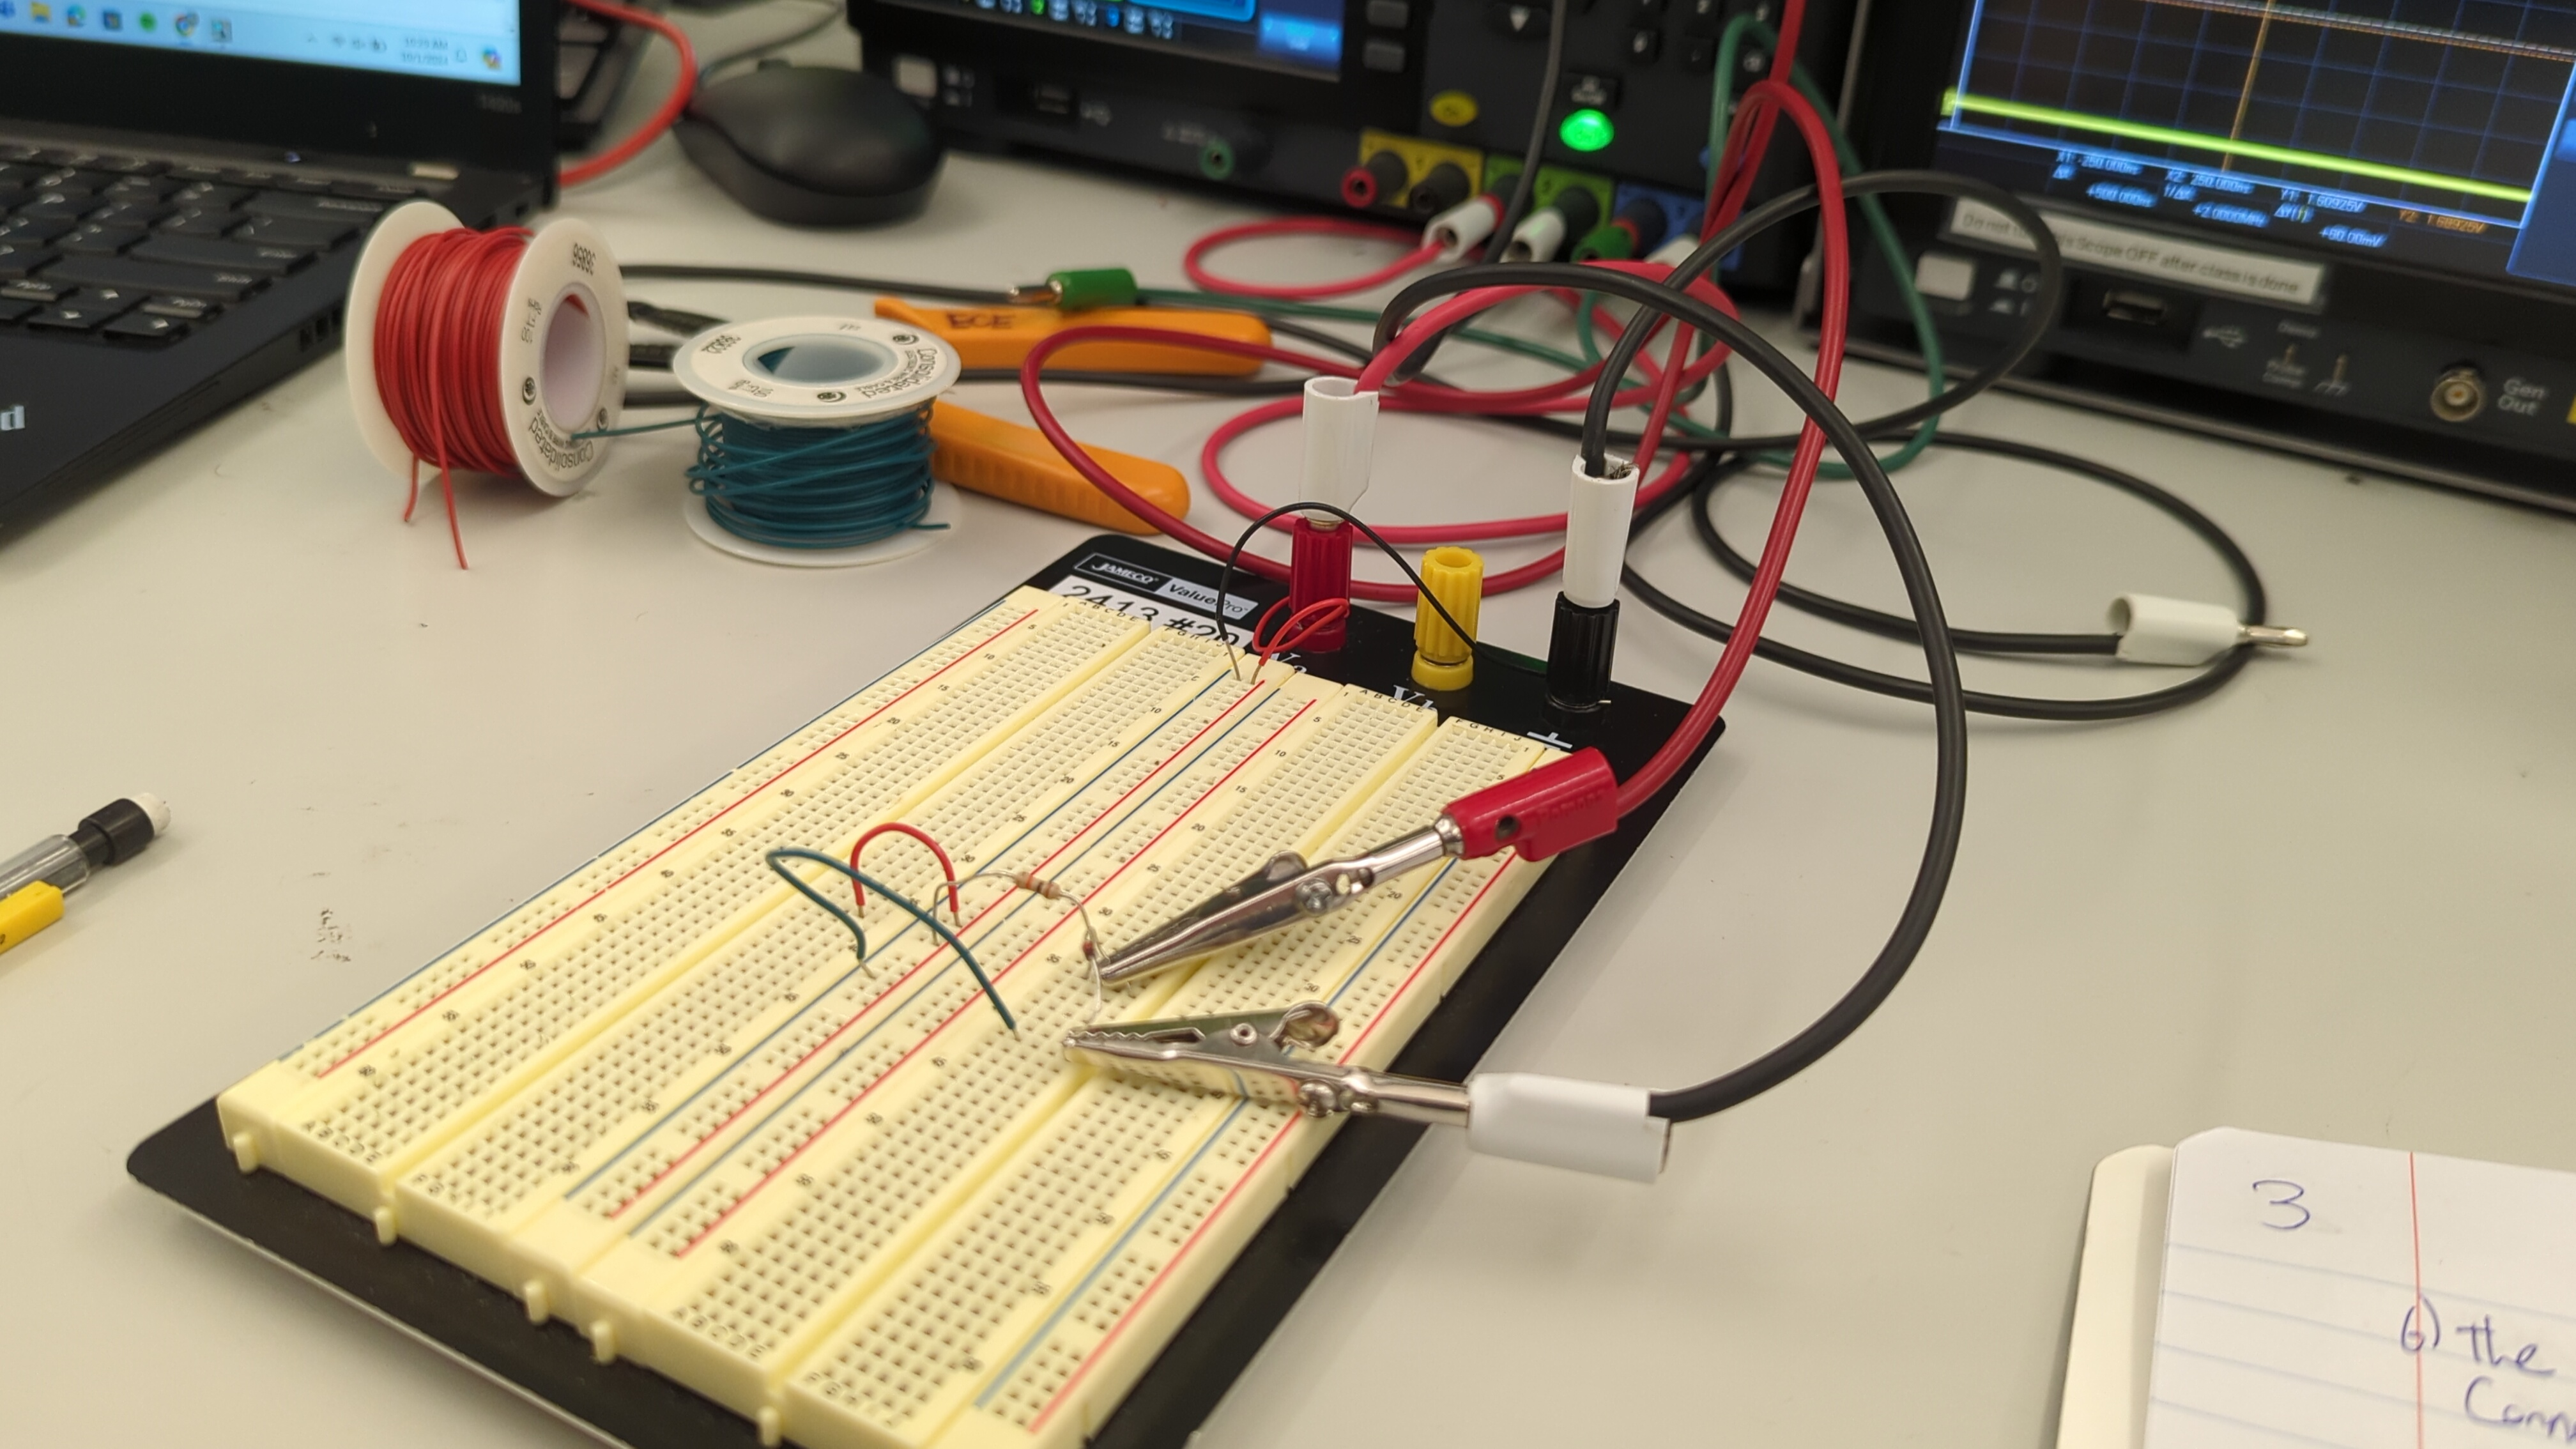
\includegraphics[width=.75\textwidth]{Figures/L2F2}
  \caption{Physical Circuit Construction}
  \label{fig:2}
\end{figure}

Then testing this circuit, the \textbf{voltage across the forward-biased diode is measured as $.6[\si{\volt}]$, and $9.99[\si{\volt}]$ for the reverse-biased diode.} We can then measure the value of the resistor to confirm it is within specification (the gold band indicates a $\pm5\%$ tolerance. The \textbf{measured resistance is} $9.938[\si{\kilo\ohm}]$, which is within the tolerance. Finally, we \textbf{measure the voltage readout as} $10.007[\si{\volt}]$, which is close to the expected value of $10[\si{\volt}]$. We may now proceed to calculate the reverse currents ($I_s$) from the taken measurements:

  $$I_D=\dfrac{V_s-V_D}{R}\to\left\{\begin{array}{ll} \dfrac{10.007-.6}{9.938k}[\si{\ampere}], &\text{in Forward-Bias}\\\\ \dfrac{10.007-9.99}{9.938k}[\si{\ampere}], &\text{in Reverse-Bias}\end{array}$$
  $$\boxed{I_D=\dfrac{V_s-V_D}{R}\to\left\{\begin{array}{ll}.9466[\si{\milli\ampere}], &\text{in Forward-Bias}\\\\ 1.7106\cdot10^{-6}[\si{\ampere}], &\text{in Reverse-Bias}\end{array}}$$

We know that the current measurement is inaccurate, as it should be 0. Thus, the current that was calculated above must be the leakage current.

    \subsubsection{Calculating $I_s$ and $n$}

    We can use the Shockley equation, or:

    $$I_D=I_se^{\frac{V_D}{nV_T}}$$

    Note: the added 1 term can be dropped, as it does not make a significant difference to the large magnitudes we are dealing with. Thus, we can use our original measurement, as well as an additional one taken at $5[\si{\volt}]$ input. Thus, we obtain:

    \begin{center}
    \begin{tabular}[H]{|c|c|c|c|}
      \hline
      Input \# & Input Voltage & Diode Voltage & Diode Current\\
      \hline
      Input 1 & $10.007[\si{\volt}]$ & $.6[\si{\volt}]$ & $.9466[\si{\milli\amp}]$\\
      \hline
      Input 2 & $5[\si{\volt}]$ & $.577[\si{\volt}]$ & $.4451[\si{\milli\amp}]$\\
      \hline
    \end{tabular}
    \end{center}

    We may now set up the equations:

    $$\left( .9466\cdot10^{-3} \right)=I_se^{\frac{.6}{(.025)n}$$
    $$\left( .4451\cdot10^{-3} \right)=I_se^{\frac{.577}{(.025)n}$$

    Solving these, we find:

    $$\boxed{n=1.22\quad\text{ and }\quad I_s=2.675\cdot10^{-12}[\si{\ampere}]}$$

    \subsubsection{Temperature Dependence}

    We now proceed to spray the diode with an aerosol refrigerant. After spraying the diode, we found that the voltage became $.76[\si{\volt}]$. From our room temperature measurement, we know that the voltage is $.6[\si{\volt}]$ at approximately $20[\si{\celsius}]$. Thus, we may find the constant:

    $$6=-.002(20)+C$$
    $$C=.64[\si{\volt}]$$

    We can now calculate the temperature response, with $V_r$ as the response voltage, using:

    $$V_r=-.002T+.64$$

    Therefore, with an output of $.76[\si{\volt}]$, the \textbf{temperature must be}:

    $$.76=-.002(T)+.64$$
    $$T=-(.12/.002)$$
    $$\boxed{T=-60[\si{\celsius}]}$$

    Applying heat by holding the diode, we \textbf{find the body temperature voltage to be} $.595[\si{\volt}]$, which gives us:

    $$.595=-.002T+.64$$
    $$T=.045/.002$$
    $$\boxed{T=22.5[\si{\celsius}]}$$

    \subsection{Using Different Diodes}

    \subsubsection{Energy Band Gaps and Diodes}

    Using a 1N34A instead of the 1N914, we measure:

    $$V_D=\left\{\begin{array}{ll} .34[\si{\volt}], & \text{In Forward-Bias}\\ 9.912[\si{\volt}], & \text{In Reverse-Bias}\end{array}$$

    Repeating similar measurements with Green and Red LEDs, respectively, we see:

    $$V_{D(grn)}=\left\{\begin{array}{ll} 1.858[\si{\volt}], & \text{In Forward-Bias}\\ 9.992[\si{\volt}], & \text{In Reverse-Bias}\end{array}$$
    $$V_{D(red)}=\left\{\begin{array}{ll} 1.626[\si{\volt}], & \text{In Forward-Bias}\\ 9.992[\si{\volt}], & \text{In Reverse-Bias}\end{array}$$

    Thus, we may conclude that the Red LED has less energy band gap, which results in less $V_{drop}$ when in forward bias mode. Similarly, we can conclude that, for the germanium diode, the energy band gap is the least by far.

    \subsubsection{Implementing Zener Diodes}

    We now swap the LEDs with a 1N4735A Zener Diode. Measuring the Diode's voltage response, we get:

    \begin{center}
    \begin{tabular}[H]{|c|c|c|c|c|c|c|c|c|c|}
      \hline
      $V^{+}[\si{\volt}]$ & 0 & 1 & 2 & 3 & 4 & 5 & 6 & 7 & 8 \\
      \hline
      $V_D[\si{\volt}]$ & 0 & .999 & 1.999 & 2.999 & 3.999 & 4.969 & 5.671 & 5.927 & 6.017\\
      \hline
    \end{tabular}
    \begin{tabular}[H]{|c|c|c|c|c|c|c|}
      \hline
      9 & 10 & 11 & 12 & 13 & 14 & 15\\
      \hline
      6.06 & 6.084 & 6.1 & 6.111 & 6.119 & 6.128 & 6.131\\
      \hline
    \end{tabular}
  \end{center}

  We may see that the implementation of a zener diode can provide useful voltage limitation properties to a circuit, oftentimes for circuit protection. 

  \subsubsection{The 1N4744A and 1N4735A}

  The breakdown voltage \textbf{was measured as roughly} $15.2[\si{\volt}]$

  Experimenting with the 1N4735A, we dissipated $5[\si{\watt}]$ of power; however, the maximum current of the diode can be found as:

  $$\frac{1[\si{\watt}]}{10[\si{\volt}]}=.1[\si{\ampere}]$$

  This is less than the passed $.5[\si{\ampere}]$, which caused the diode to break down. Adding a LED, we found that it began glowing once the current was greater than the $.1[\si{\ampere}]$, indicating that too much voltage is dissipated in the resistor, so the zener diode must go into breakdown to supply the needed current to the LED. Still, it was quite dim, meaning it most likely needs more current than it was receiving (it would need more than $.1[\si{\ampere}]$.

\section{Conclusion}


\end{document}
